%TC:ignore
Several validation tests, in accordance with  were conducted for this research. Their outputs are shown in this chapter. We start presenting our findings on the extreme conditions test, then we show the results of the sensitivity analysis, and we conclude this chapter by comparing the data of the model to real-world values.

\subsection{Extreme conditions test}
\label{s:extreme_conditions}
To test the structure of the model, we subjected it to extreme conditions to evaluate if the model behaves accordingly. Figures~\ref{fig:temp_fly} to~\ref{fig:reproduction_meat} show the results.

\begin{figure}[h!]
    \centering
    \begin{minipage}{0.45\textwidth}
        \centering
        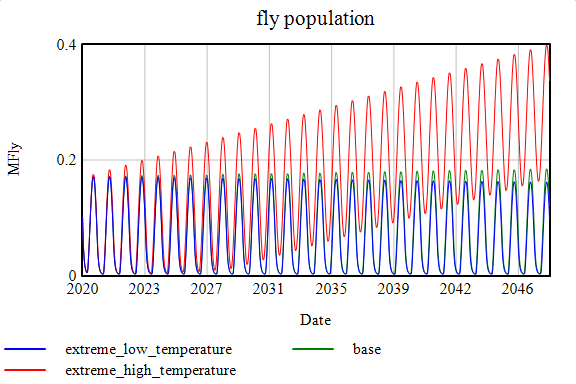
\includegraphics[width=\textwidth]{images/extremes/Temperature_fly_population.png} 
        \caption{Effect of extreme temperature increase values on fly population}
        \label{fig:temp_fly}
    \end{minipage}
    \begin{minipage}{0.45\textwidth}
        \centering
        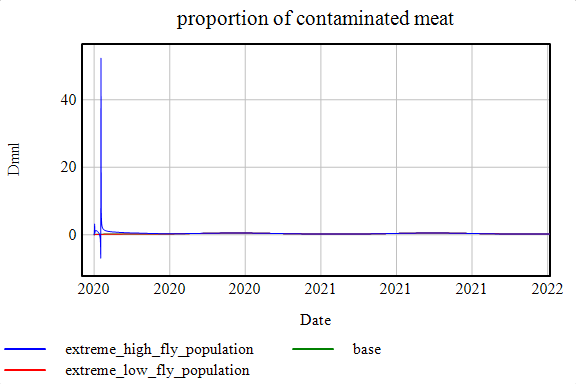
\includegraphics[width=\textwidth]{images/extremes/Fly_population_contaminated_meat.png} 
        \caption{Effect of extreme initial fly population values on proportion of contaminated meat}
        \label{fig:fly_meat}
    \end{minipage}
\end{figure}

\begin{figure}[h!]
    \centering
    \begin{minipage}{0.45\textwidth}
        \centering
        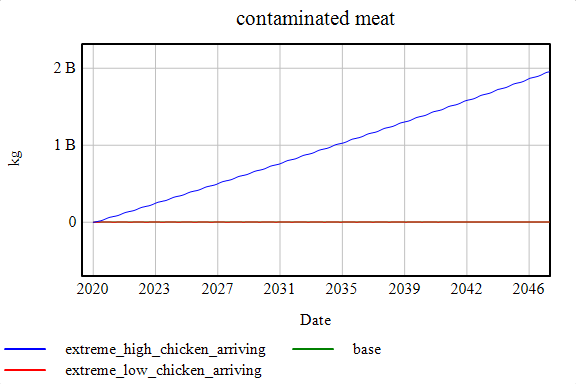
\includegraphics[width=\textwidth]{images/extremes/Chicken_arriving_contaminated_meat.png} 
        \caption{Effect of extreme chicken arriving to hatcheries values on contaminated meat}
        \label{fig:chicken_meat}
    \end{minipage}
    \begin{minipage}{0.45\textwidth}
        \centering
        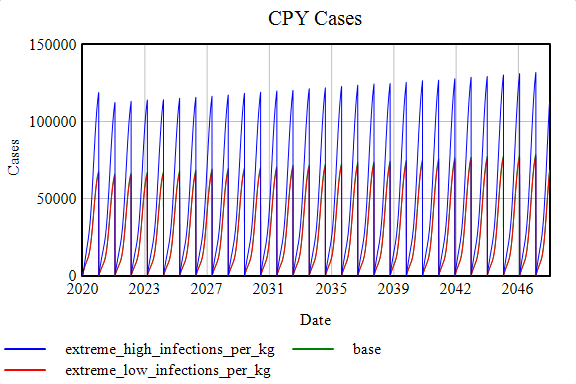
\includegraphics[width=\textwidth]{images/extremes/Infections_per_kg_CPY_cases.png} 
        \caption{Effect of extreme values of infections per kg of meat consumed on Campylobacteriosis cases}
        \label{fig:infections_cases}
    \end{minipage}
\end{figure}

\begin{figure}[h!]
    \centering
    \begin{minipage}{0.45\textwidth}
        \centering
        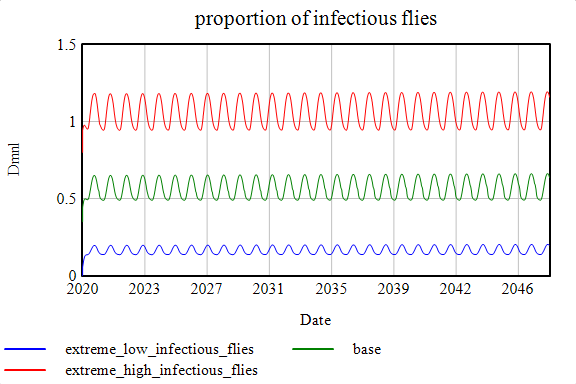
\includegraphics[width=\textwidth]{images/extremes/base_infectious_flies_proportion_flies.png} 
        \caption{Effect of extreme base infectious flies values on proportion of infected flies}
        \label{fig:fly_meat}
    \end{minipage}
    \begin{minipage}{0.45\textwidth}
        \centering
        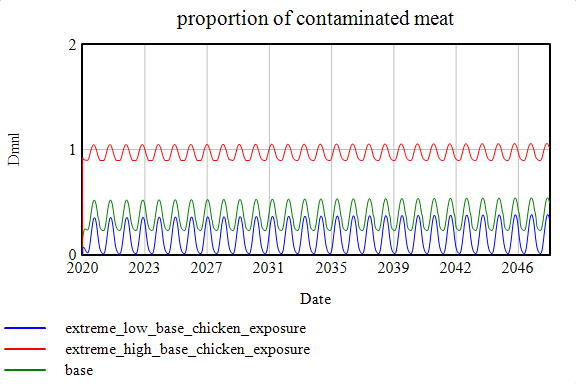
\includegraphics[width=\textwidth]{images/extremes/Base_chicken_exposure_contaminated_meat.png} 
        \caption{Effect of extreme base chicken exposure rates on proportion of contaminated meat}
        \label{fig:exposure_meat}
    \end{minipage}
\end{figure}

\begin{figure}[h!]
    \centering
    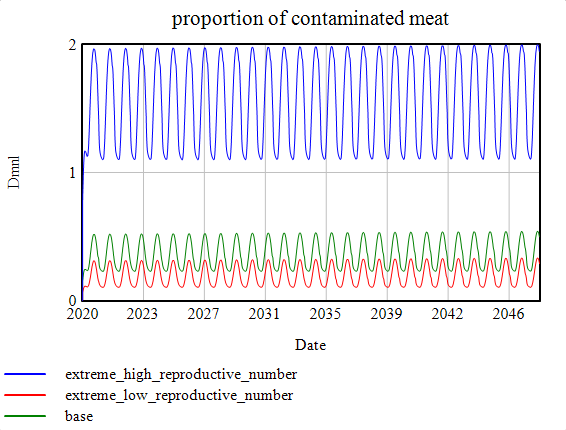
\includegraphics[width=0.45\textwidth]{images/extremes/CPY_reproduction_contaminated_meat.png} 
    \caption{Effect of extreme CPY reproduction on proportion of contaminated meat}
    \label{fig:reproduction_meat}
\end{figure}

%The extreme high value of temperature increase evidences a problem in the model, as fly reproduction is unreasonably high since extreme temperatures are likely to create a harsher environment for them as well. For the extreme high values of initial fly population and base infectious flies, the model reports a proportion of contaminated meat that is greater than the total amount of meat, which should not be possible. A similar thing happens with base infections flies and base chicken exposure rate, which can cause more infectious flies than there are total flies. When chicken arriving from hatcheries are decreased (and thus made lower than the demand), the model can handle the situation because it does not allow for consumption of more chicken that are available, but when instead it is raised, the excess supply is never dumped, creating an issue of accumulating meat indefinitely which is not realistic. Lastly, when infections per kg of meat consumed are raised 20 times its original value, it can bring issues of too many people being infected, since our model does not account for immunity of population, all population is indefinitely susceptible which becomes a problem when infection numbers are very big.


\subsection{Multivariate analysis}

We ran multivariate analysis to account for the compounded effect of different uncertainties, and the results can be found in figures \ref{fig:multi_coi}, \ref{fig:multi_meat}, \ref{fig:multi_chicken}, and \ref{fig:multi_human}. The observed change is mostly regarding numerical sensitivity, but we can see that the contaminated chicken meat can overshoot at times, which is the result of people refusing to eat meat as a result of increased infections, but the chicken were already in the production cycle so there was excess production.

% ADD HOW MANY RUNS

\begin{figure}[h!]
    \centering
    \begin{minipage}{0.45\textwidth}
        \centering
        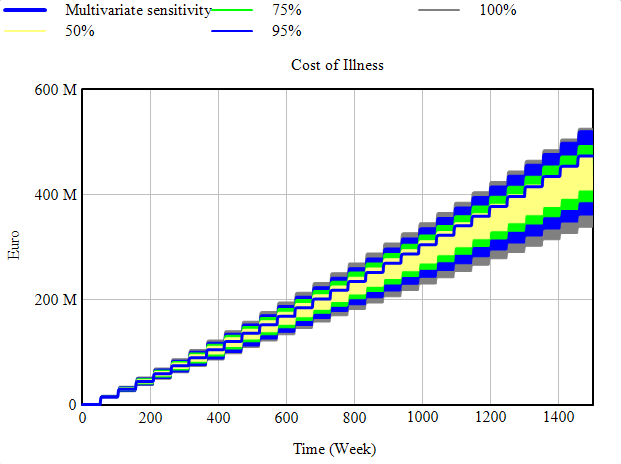
\includegraphics[width=1\textwidth]{images/sensitivity/Multivariate COI.png} % first figure itself
        \caption{Cost of Illness in the multivariate analysis}
        \label{fig:multi_coi}
    \end{minipage}\hfill
    \begin{minipage}{0.45\textwidth}
        \centering
        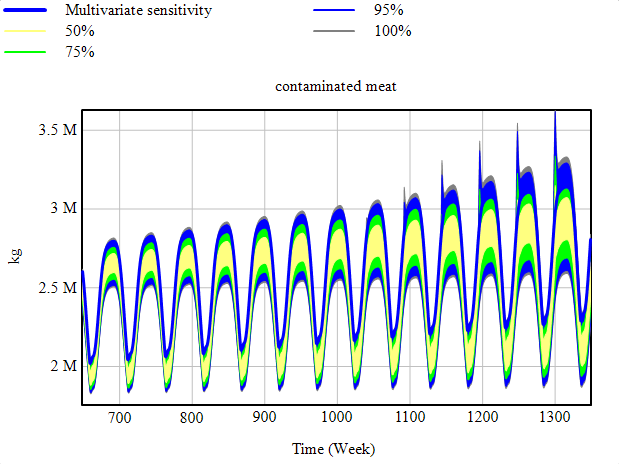
\includegraphics[width=1\textwidth]{images/sensitivity/Multivariate contaminated meat.png} % second figure itself
        \caption{Contaminated chicken meat in the multivariate analysis}
        \label{fig:multi_meat}
    \end{minipage}
\end{figure}

\begin{figure}[h!]
    \centering
    \begin{minipage}{0.45\textwidth}
        \centering
        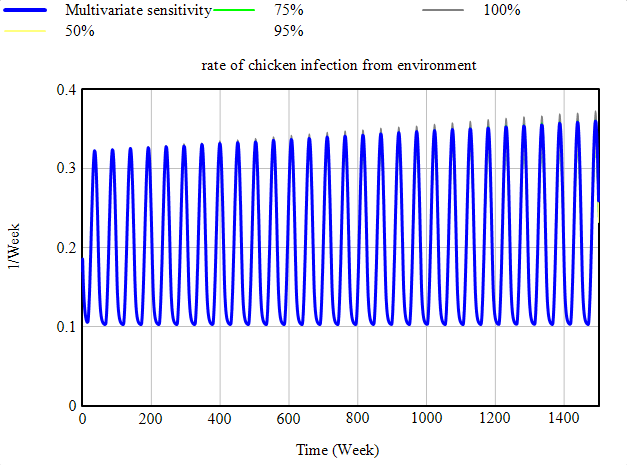
\includegraphics[width=1\textwidth]{images/sensitivity/Multivariate chicken infection.png} 
        \caption{Chicken infections from environment in the multivariate analysis}
        \label{fig:multi_chicken}
    \end{minipage}\hfill
    \begin{minipage}{0.45\textwidth}
        \centering
        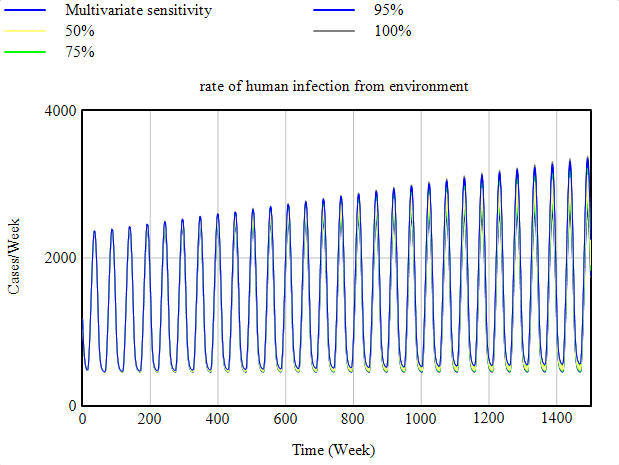
\includegraphics[width=1\textwidth]{images/sensitivity/Multivariate human infection.png}
        \caption{Human infections from environment in the multivariate analysis}
        \label{fig:multi_human}
    \end{minipage}
\end{figure}


\subsection{Sensitivity Analysis}
\subsubsection{Population scenarios}

Based on population projections \parencite{nidi_nidi_2020} we ran the sensitivity analysis and got the results in figures \ref{fig:pop_coi}, \ref{fig:pop_meat}, \ref{fig:pop_chicken}, and \ref{fig:pop_human}. Because a population increase also increases demand for chicken, generating a reaction across the model than can be appreciated in the increased contaminated chicken meat stock as well. Because more people get infected in total and present symptoms, the cost of illness also increases.

\begin{figure}[h!]
    \centering
    \begin{minipage}{0.45\textwidth}
        \centering
        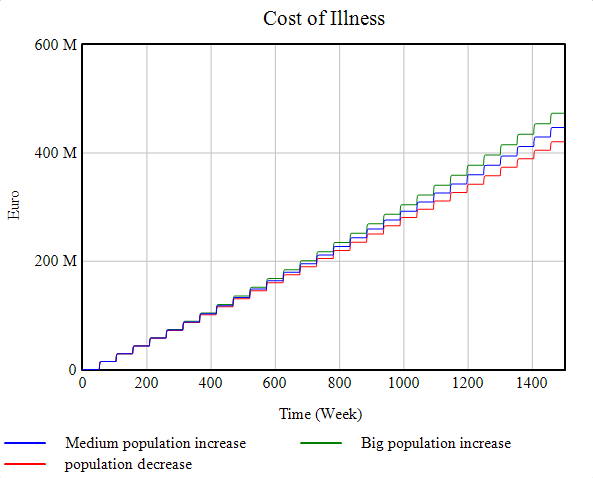
\includegraphics[width=1\textwidth]{images/sensitivity/Population COI.png} % first figure itself
        \caption{Cost of Illness in the different population scenarios}
        \label{fig:pop_coi}
    \end{minipage}\hfill
    \begin{minipage}{0.45\textwidth}
        \centering
        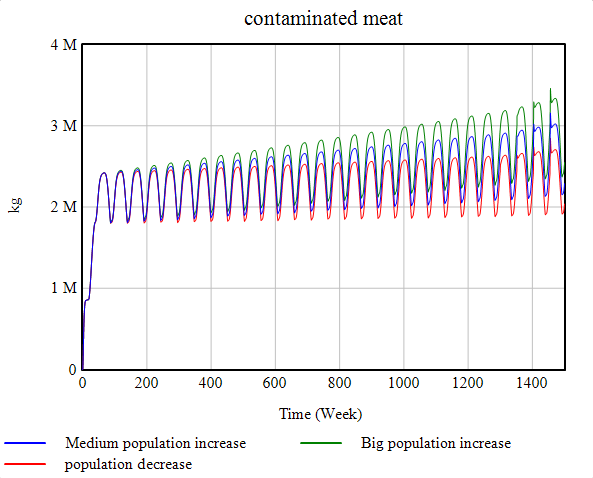
\includegraphics[width=1\textwidth]{images/sensitivity/Population contaminated meat.png} % second figure itself
        \caption{Contaminated chicken meat in the different population scenarios}
        \label{fig:pop_meat}
    \end{minipage}
\end{figure}

\begin{figure}[h!]
    \centering
    \begin{minipage}{0.45\textwidth}
        \centering
        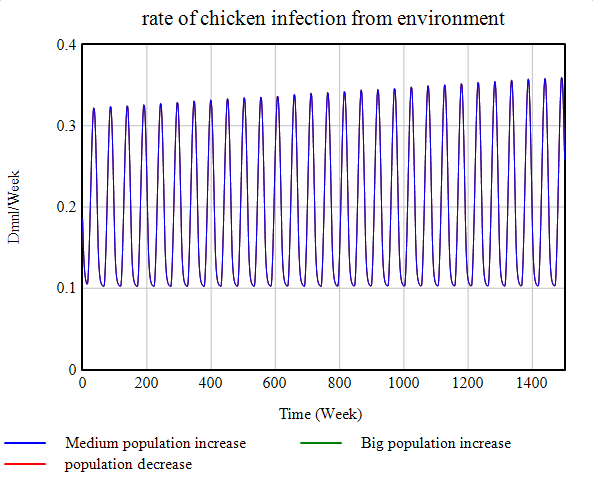
\includegraphics[width=1\textwidth]{images/sensitivity/Population chicken infection.png} 
        \caption{Chicken infections from environment in the different population scenarios}
        \label{fig:pop_chicken}
    \end{minipage}\hfill
    \begin{minipage}{0.45\textwidth}
        \centering
        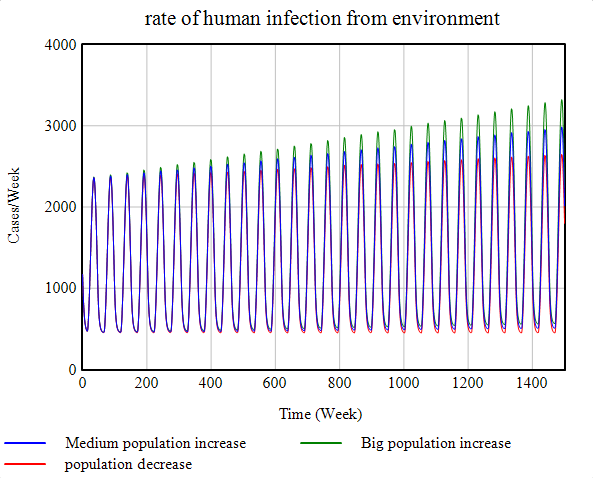
\includegraphics[width=1\textwidth]{images/sensitivity/Population human infection.png}
        \caption{Human infections from environment in the different population scenarios}
        \label{fig:pop_human}
    \end{minipage}
\end{figure}

\subsubsection{Climate scenarios}

% EXPLICITLY MENTION THIS IS UNIVARIATE

\textbf{Average temperature increase}

Based on climate change projections \parencite{knmi_knmi_2015} we ran the sensitivity analysis and got the results in figures \ref{fig:temp_coi}, \ref{fig:temp_meat}, \ref{fig:temp_chicken}, and \ref{fig:temp_human}. Temperature increasing aids in the development of disease vectors, which has a direct impact on human infections, besides also affecting indirectly through the food borne route of transmission. This results in increased cost of illness proportional to the increase in temperature over the years.

\begin{figure}[h!]
    \centering
    \begin{minipage}{0.45\textwidth}
        \centering
        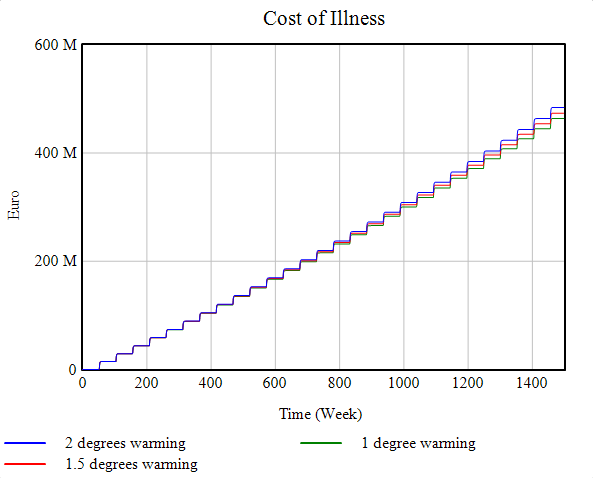
\includegraphics[width=1\textwidth]{images/sensitivity/Temperature projection COI.png} % first figure itself
        \caption{Cost of Illness in the different temperature increase scenarios}
        \label{fig:temp_coi}
    \end{minipage}\hfill
    \begin{minipage}{0.45\textwidth}
        \centering
        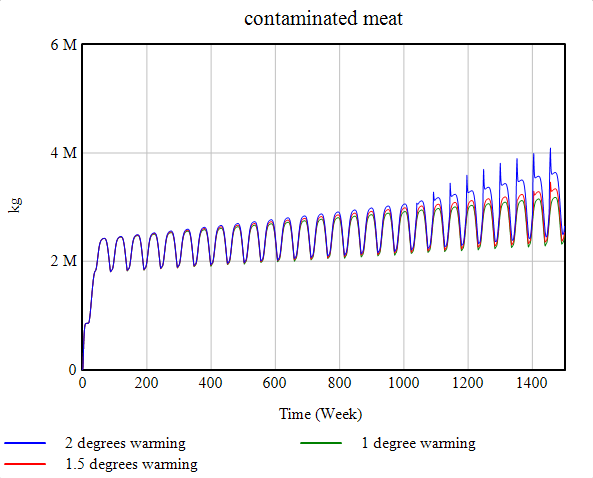
\includegraphics[width=1\textwidth]{images/sensitivity/Temperature projection contaminated meat.png} % second figure itself
        \caption{Contaminated chicken meat in the different temperature increase scenarios}
        \label{fig:temp_meat}
    \end{minipage}
\end{figure}

\begin{figure}[h!]
    \centering
    \begin{minipage}{0.45\textwidth}
        \centering
        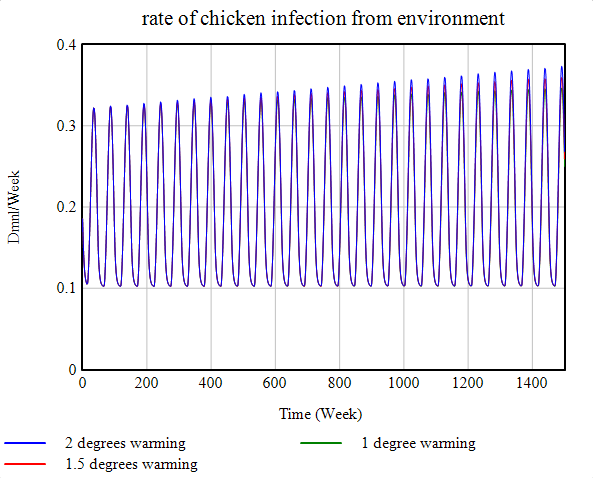
\includegraphics[width=1\textwidth]{images/sensitivity/Temperature projection chicken infection.png} 
        \caption{Chicken infections from environment in the different temperature increase scenarios}
        \label{fig:temp_chicken}
    \end{minipage}\hfill
    \begin{minipage}{0.45\textwidth}
        \centering
        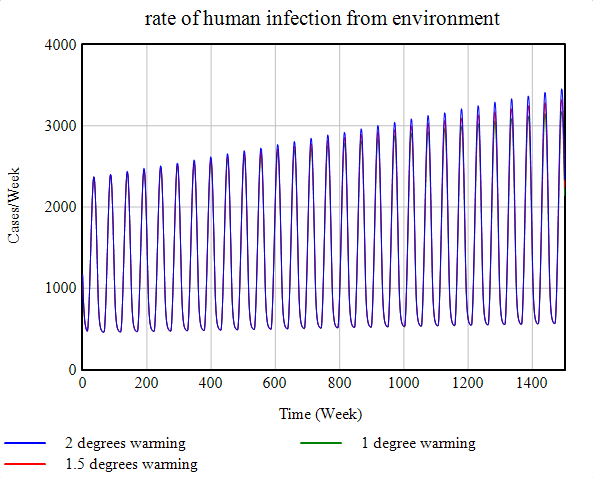
\includegraphics[width=1\textwidth]{images/sensitivity/Temperature projection human infection.png}
        \caption{Human infections from environment in the different temperature increase scenarios}
        \label{fig:temp_human}
    \end{minipage}
\end{figure}

\textbf{Seasonal temperature increase}

There is uncertainty in how the temperature might increase in the future. It seems that the increase is not uniform throughout the year, but that instead summers might warm up faster than winters. We modelled this uncertainty and compared the scenarios. The seasonal variation in temperature increase leads to longer warmer periods compared to cold periods, which also affects disease vector propagation and has an impact in infections and subsequently in the cost of illness. This can be appreciated in figures. \ref{fig:season_coi}, \ref{fig:season_meat}, \ref{fig:season_chicken}, and \ref{fig:season_human}.

\begin{figure}[h!]
    \centering
    \begin{minipage}{0.45\textwidth}
        \centering
        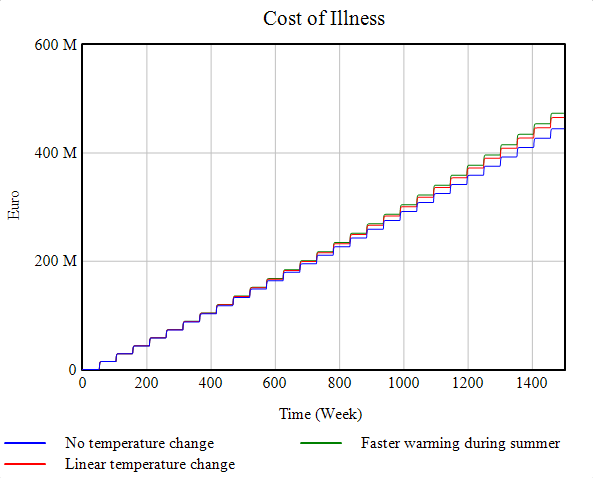
\includegraphics[width=1\textwidth]{images/sensitivity/Seasonal temperature COI.png} % first figure itself
        \caption{Cost of Illness in the different temperature seasonality scenarios}
        \label{fig:season_coi}
    \end{minipage}\hfill
    \begin{minipage}{0.45\textwidth}
        \centering
        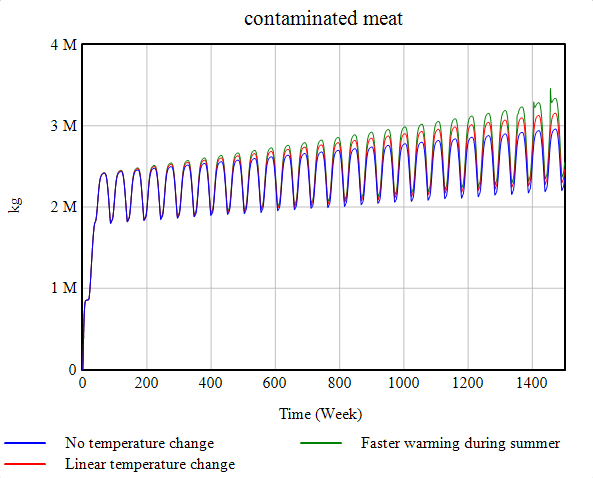
\includegraphics[width=1\textwidth]{images/sensitivity/Seasonal temperature contaminated meat.png} % second figure itself
        \caption{Contaminated chicken meat in the different temperature seasonality scenarios}
        \label{fig:season_meat}
    \end{minipage}
\end{figure}

\begin{figure}[h!]
    \centering
    \begin{minipage}{0.45\textwidth}
        \centering
        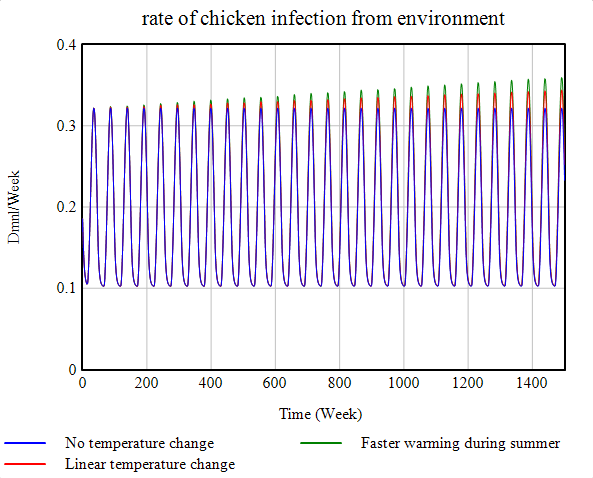
\includegraphics[width=1\textwidth]{images/sensitivity/Seasonal temperature chicken infection.png}
        \caption{Chicken infections from environment in the different temperature seasonality scenarios}
        \label{fig:season_chicken}
    \end{minipage}
    \begin{minipage}{0.45\textwidth}
        \centering
        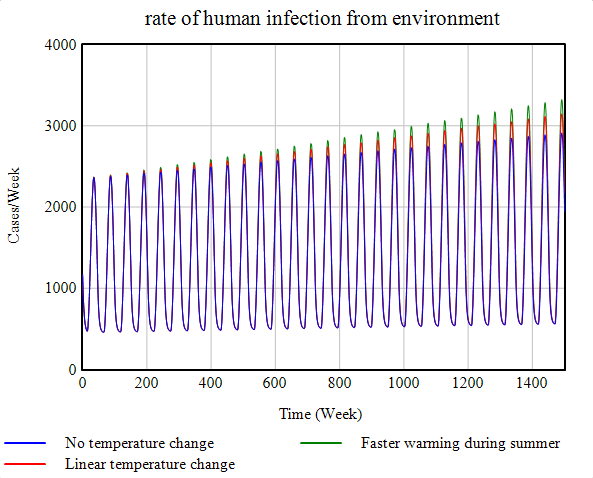
\includegraphics[width=1\textwidth]{images/sensitivity/Seasonal temperature human infection.png}
        \caption{Human infections from environment in the different temperature seasonality scenarios}
        \label{fig:season_human}
    \end{minipage}
\end{figure}

\subsubsection{Public health scenarios}

On figure \ref{fig:symptom_COI} we can see the result of rate of symptomatic infections changing, which is a behaviour that has been observed recently \parencite{medema_assessment_1996}. This only bring changes to the cost of illness, as infections remain the same across the model, but the severity of the disease requires more treatment.

\begin{figure}[h!]
    \centering
    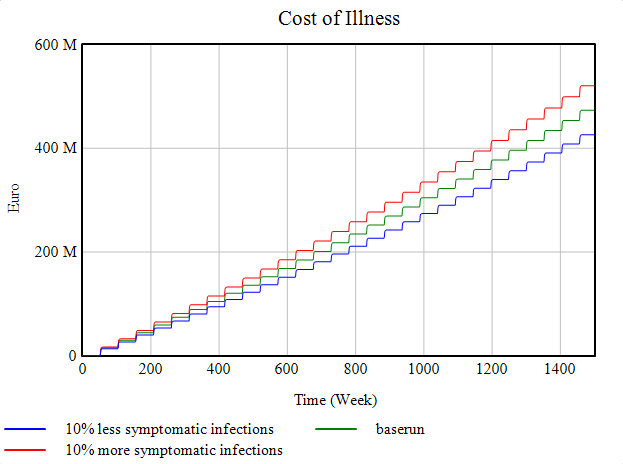
\includegraphics[width=0.45\textwidth]{images/extremes/Symptomatic COI.png} 
    \caption{Cost of illness in the different symptomatic infection scenarios}
    \label{fig:symptom_COI}
\end{figure}

\subsection{Comparison to real world data}

\textcite{vlaanderen_staat_2019} estimated there were around 71.000 cases of Campylobacteriosis in the Netherlands in 2018, 67.000 in 2017 and 79.000 in 2016. We plotted the amount of cases produced by our model against the average of these three values. The results can be seen in Figure~\ref{fig:val_human_cases}. We can see the stock in our model is a good reflection of the real world. 

\textcite{nepluvi_rapportage_2019} monstered broiler chickens weekly in 2018, and found $41,9$-$58.1\%$ of broiler chickens were tested positive for \textit{Campylobacter}. This concerns chickens from slaughterhouses. As can be seen in Figure~\ref{fig:val_chickens}, our base model has similar values for each year.

In the Netherlands the (unsanitary) preparation and/or consumption of chicken were attributed to $20$-$30\%$ of infections in 2018. However, around $50$-$80\%$ of cases can be attributed to \textit{Campylobacter} strains associated with poultry \parencite{cuperus_surveillance_2020, nepluvi_rapportage_2019}. Therefore, it is safe to assume that there are multiple transmission routes. We assume the biggest transmission routes can be found in the environment. In the base model, around 5.70\% of the infections stem from the preparation and/or consumption of chicken. This can be seen in Figure~\ref{fig:val_sources}. It may be the case that the environment plays a bigger role than we previously assumed, after all, it is easier to trace back the cause to undercooked meat than to a wild bird.

Numbers on the average amount of chicken meat consumption per Dutch person differ, but they are between 0.22 and 0.47 kg of chicken meat per week~\parencite{schotman_europese_2018, waveningen_university__research_we_2020}. In our model this fluctuates between 0.153 and 0.203 so there is a slight discrepancy.

We also validated our DALYs and Cost of Illness against the data points from \parencite{mangen_campylobacteriosis_2007}. Note that these values are from 2007. As can be seen in Figure~\ref{fig:val_dalys} our model determines higher DALYs than given in the literature. This may indicate that there are more chronic diseases that can be traced back to \textit{Campylobacter} than is currently happening in the real world. Perhaps the specialists are overlooking the bacterium as a cause, or they are simply unable to pinpoint the cause.

In Figure~\ref{fig:val_coi} it can be seen that the Cost of Illness calculated by the model is lower than \citeauthor{mangen_campylobacteriosis_2007}'s values. This is probably due to the fact that we only look at 3 chronic conditions and the acute conditions. 

It is estimated there are around 17 million species of \textit{Diptera} per person \parencite{gorman_trillions_2017}. We are only interested in \textit{Musca domestica}. It is unknown what their numbers are in the Netherlands, and we are unable to estimate. However, it has been guessed that the population of Houseflies will increase by 244\% by 2080 \parencite{mcalister_secret_2017}. In The amount of flies in our model after 1 year is 20.000 of which 7.700 are infectious (TIME STEP = 0.0625). This is probably not a proper reflection of the real world, but one can assume that it is only 7.700 flies that have directly caused a disease in humans and/or chickens.

The model also includes an Infection risk from birds (2.5e-05). There are about 1.3 million birds in the Netherlands \parencite{noauthor_miljoenen_2019}. There was no literature on the risk from birds, so we assumed a somewhat safe value. We doubt \textit{Campylobacter} will ever be exterminated due to the presence of these environmental factors, even if we are somehow able to keep our farms, slaughterhouses and stores free from \textit{Campylobacter}.



\begin{figure*}[!h]
    \centering
    \begin{minipage}{0.45\textwidth}
        \centering
        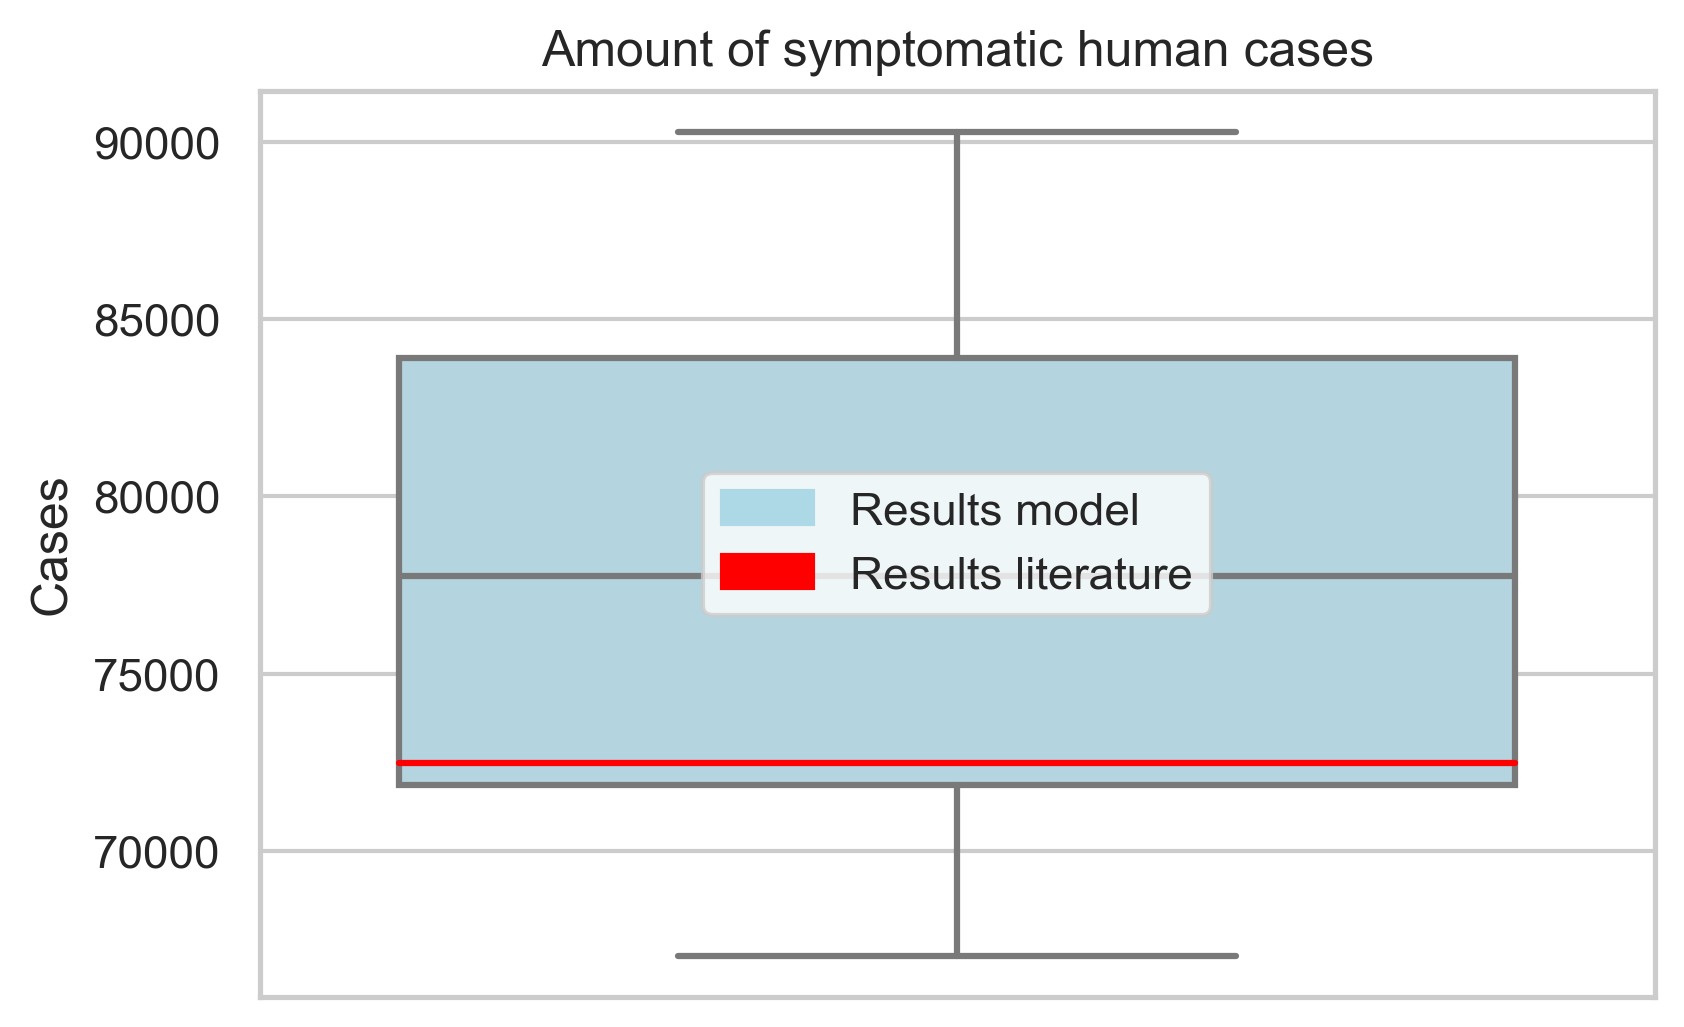
\includegraphics[width=0.9\textwidth]{notebooks/human_cases2.png} % first figure itself
        \caption{Validation of human cases}
        \label{fig:val_human_cases}
    \end{minipage}\hfill
    \begin{minipage}{0.45\textwidth}
        \centering
        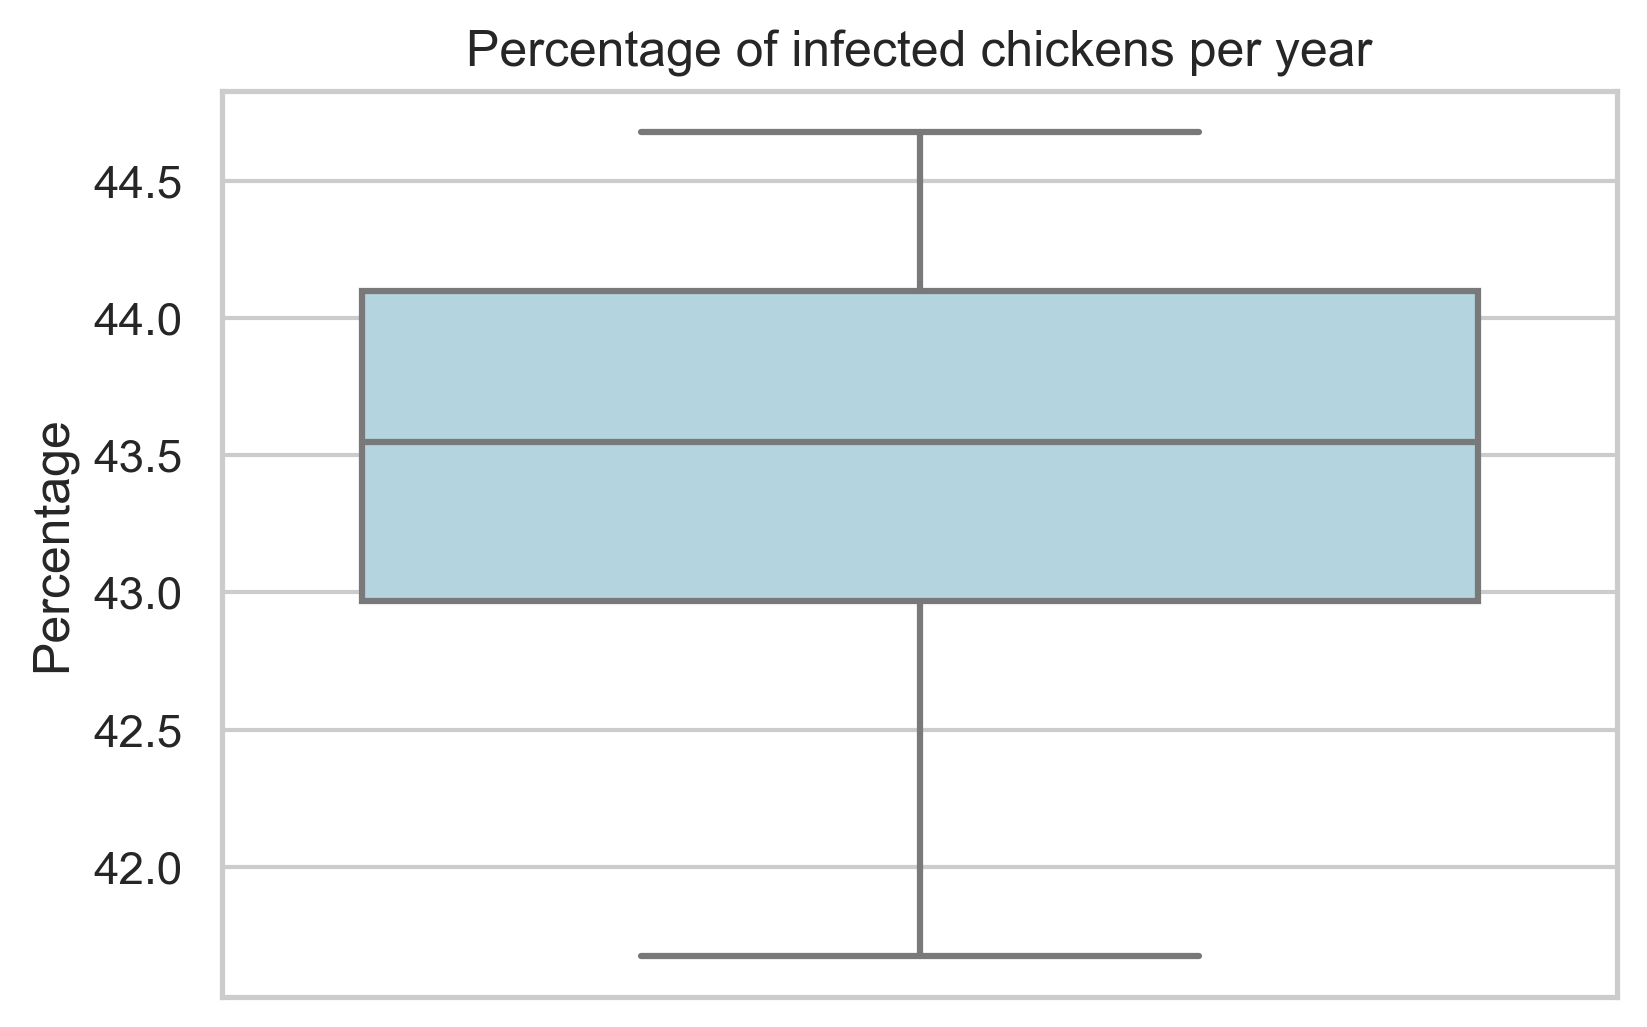
\includegraphics[width=0.9\textwidth]{notebooks/chickens2.png} % second figure itself
        \caption{Validation of proportion infected chickens}
	    \label{fig:val_chickens}
    \end{minipage}
\end{figure*}

\begin{figure*}[!h]
	\centering
	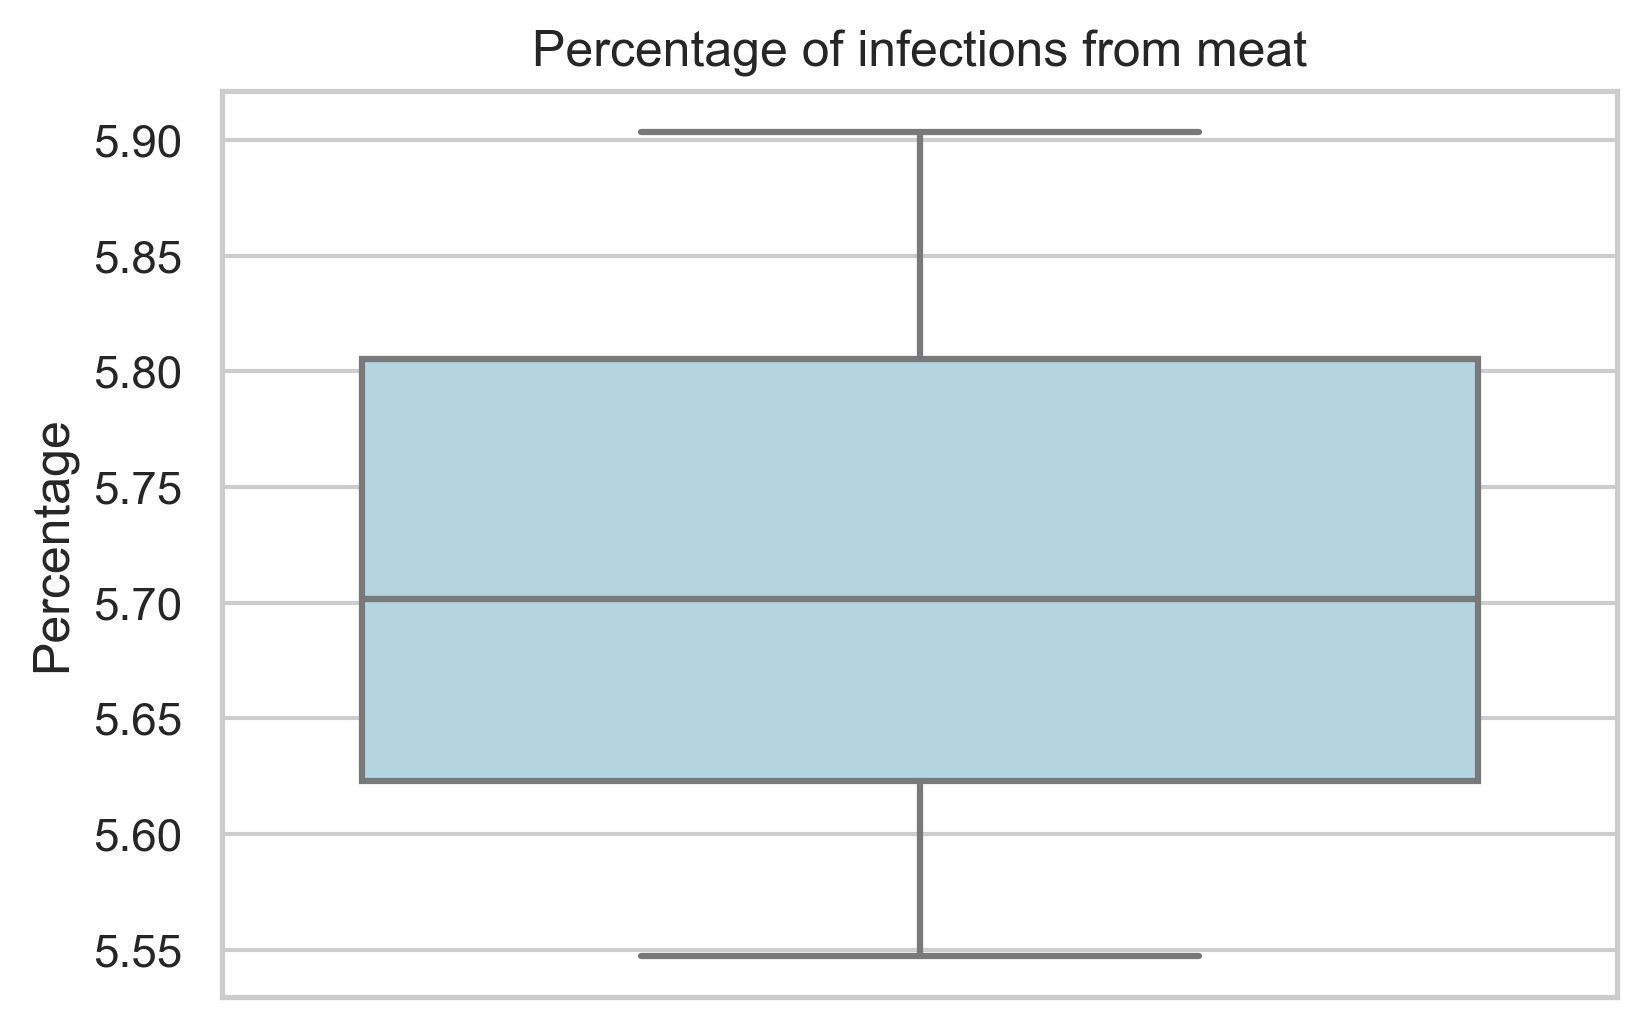
\includegraphics[width=0.5\textwidth]{notebooks/source2.png}
	\caption{Validation of sources of Campylobacteriosis}
	\label{fig:val_sources}
\end{figure*}

\begin{figure*}[!h]
    \centering
    \begin{minipage}{0.45\textwidth}
        \centering
        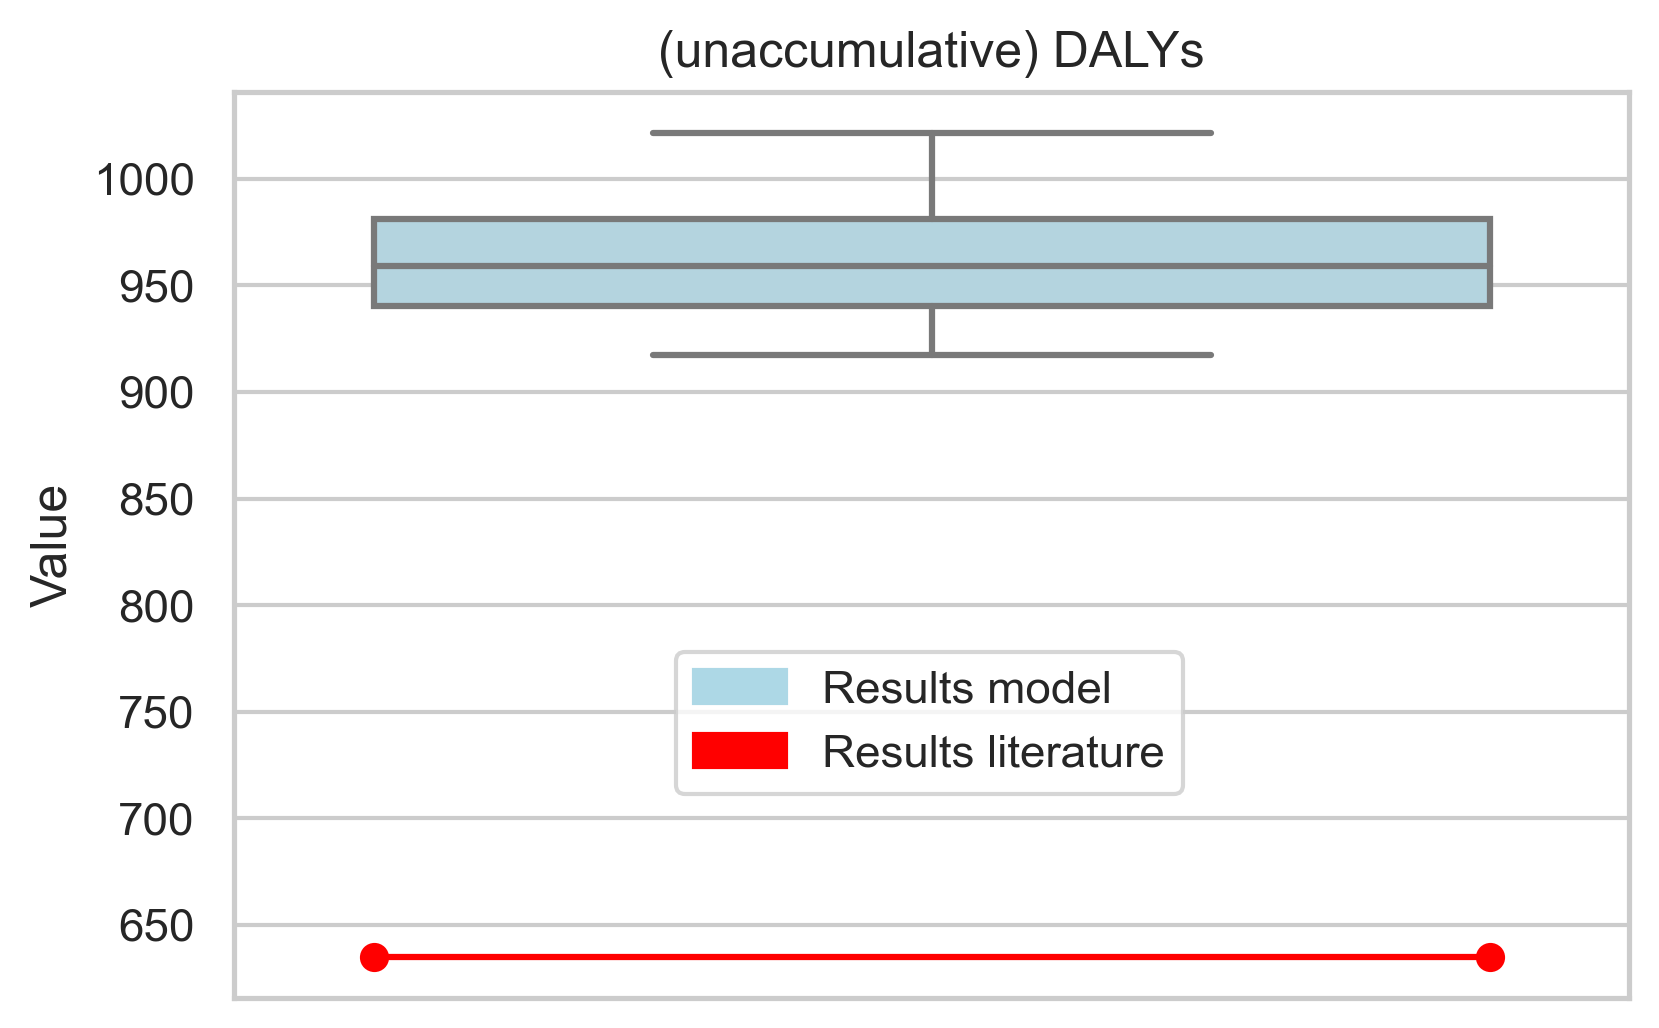
\includegraphics[width=0.9\textwidth]{notebooks/dalys2.png} % first figure itself
        \caption{Validation of DALYs}
	    \label{fig:val_dalys}
    \end{minipage}\hfill
    \begin{minipage}{0.45\textwidth}
        \centering
        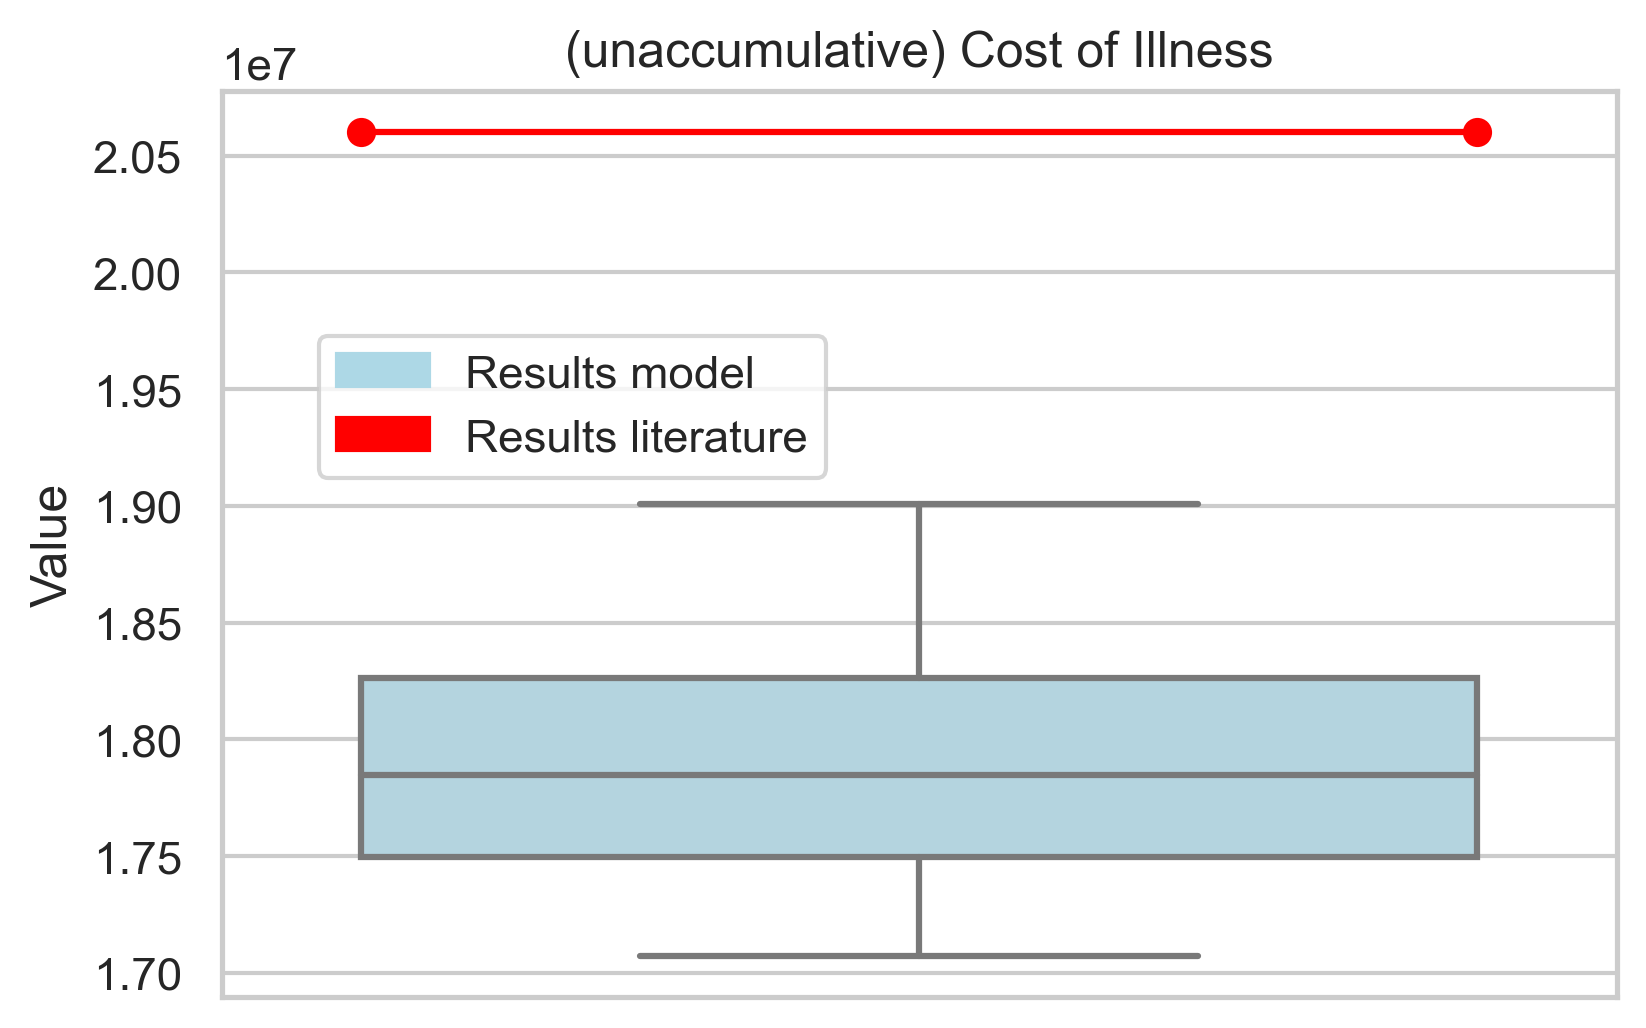
\includegraphics[width=0.9\textwidth]{notebooks/coi2.png} % second figure itself
        \caption{Validation of Cost of Illness}
	    \label{fig:val_coi}
    \end{minipage}
\end{figure*}

%TC:endignore